\documentclass[conference]{IEEEtran}
\IEEEoverridecommandlockouts
% The preceding line is only needed to identify funding in the first footnote. If that is unneeded, please comment it out.
\usepackage{cite}
\usepackage{amsmath,amssymb,amsfonts}
\usepackage{algorithmic}
\usepackage{graphicx}
\usepackage{textcomp}
\usepackage{xcolor}
\begin{document}

\title{Dynamic Load Balancing for Particle-in-Cell, CFD, and Discrete Event Simulations\\
\thanks{
This research was supported by the U.S. Department of Energy, Office of
Science, Office of Advanced Scientific Computing Research, under award
DE-AC52-07NA27344 (FASTMath SciDAC Institute) and by the National Science
Foundation under Grant No.  ACI 1533581, (SI2-SSE: Fast Dynamic Load
Balancing Tools for Extreme Scale Systems).
Any opinions, findings, and conclusions or recommendations expressed in this
material are those of the author(s) and do not necessarily reflect the views
of the National Science Foundation.
}}

\author{\IEEEauthorblockN{1\textsuperscript{st} Gerrett Diamond}
\IEEEauthorblockA{\textit{SCOREC} \\
\textit{Rensselaer Polytechnic Institute}\\
Troy, NY\\
diamog@rpi.edu}
\and
\IEEEauthorblockN{2\textsuperscript{nd} Cameron W. Smith}
\IEEEauthorblockA{\textit{SCOREC} \\
\textit{Rensselaer Polytechnic Institute}\\
Troy, NY\\
smithc11@rpi.edu}
\and
\IEEEauthorblockN{3\textsuperscript{rd} Mark S. Shephard}
\IEEEauthorblockA{\textit{SCOREC} \\
\textit{Rensselaer Polytechnic Institute}\\
Troy, NY\\
shephard@rpi.edu}
}

\maketitle

\begin{abstract}
  Extracting performance from simulations with complex information dependencies
  on massively parallel computers requires the computational work to be evenly
  distributed across the processing resources while maintaining low
  communication costs.
  Particle-in-cell and unstructured mesh-based finite element and volume
  simulations present two distinct sets of distribution requirements.
  To meet these needs, we present EnGPar's diffusive partition improvement
  method.
  EnGPar's performance is compared against XYZ (PIC?) and ParMETIS.
  Specifically, partition improvement results are provided on
  up to QRS and XYZ processes of the ABC and DEF systems, respectively.
\end{abstract}

\begin{IEEEkeywords}
partition improvement,multigraph,hypergraph,dynamic load balancing,
particle in cell, computational fluid dynamics
\end{IEEEkeywords}

\section{Introduction}

\begin{itemize}
\item motivate dynamic load balancing
\item talk about how different applications have different partitioning needs
\item Mention that engpar is general to support a range of structures.
\end{itemize}

\section{EnGPar}

%\begin{itemize}
%\item Discuss the Ngraph in general graph terms with some figures
%\item Discuss the construction for a element-partitioned mesh as an example with figure
%\item Discuss dynamic load balancing and the general diffusive steps
%\end{itemize}

EnGPar~\cite{engparSC17,engpar_github} is a tool for partition improvement and
dynamic load balancing.
EnGPar utilizes a multi-hypergraph, called the N-graph, to represent the data of
an application in a relational format that allows load balancing of the vertices
and edges simultaneously.
The N-graph is defined as $G^n = \{V, H^n, P^n\}$ where
$V$ is the set of vertices in the graph. The vertices are uniquely assigned to a single
process and are used to represent the main source of data in an application.
$H^n = \{H_1, ..., H_n\}$ are sets of hyperedges where each hyperedge connects a
subset of vertices in $V$. The pins, $P^n = \{P_1,...,P_n\}$, represent the connections from
vertices to hyperedges. Each application that utilizes EnGPar represents the data
that needs partitioning as an N-graph before running any of the partitioning tools.
The general design of the N-graph allows easy representation for different applications
that use structures such as meshes, graphs, and other relational structures.

EnGPar's partition improvement is driven by local diffusive techniques that migrate weight
from heavily weighted parts to lightly weighted parts. This is done by iteratively running
a set of steps until the target imbalance is met or no further improvements can be met.
A diffusive iteration consists of three steps: targeting, selection, and migration.
The targeting step consists of gathering information about the current partiton and deciding
which neighbors should be sent weight and how much weight to send. The selection step constructs
a plan of what vertices should be sent to each neighbor in order to satisfy the weights in
the targeting step. The final step, migration, is where the vertices are sent to their
destinations and the partition is changed.

\section{Phasta}

\begin{itemize}
\item Describe the vertex>elm problem
\item Describe the ngraph for element-partitioned meshes
\end{itemize}

\section{Particle In Cell}

%\begin{itemize}
%\item Briefly discuss PIC/XGCM
%\item Mention that the mesh partition is static.
%\item Describe the buffer/safe zone
%\item Describe the weight diffusion algorithm.
%\end{itemize}

{\color{red} How much can I talk about XCG? Assuming I should only mention XGCm.}
Particle in cell (PIC) methods are mesh applications that utilize particles in the spacial domain
of the mesh. PIC applications have additional partitioning challenges since the mesh topology
must be well balanced as well as the particles. In addition, the particles move around the mesh
and, depending on the application, may require migrating to new processes. As these simulations
continue the particles become imbalanced and will degrade performance.

XGCm, a PIC application that is a mesh oriented version of XGC, uses a 2D mesh that
{\color{red} CWS Describe a little of XGCm?}. The partitioning of the mesh is controlled
by flux faces which are geometric model faces. Each part consists of
the mesh entities within a geometric model face and several buffer layers of elements around the
model edges. The first few layers of the buffered elements are marked as a safe region as well as
the elements within the flux face. This partitioning is static and does not change during the
simulation. Particles exist within the safe elements of a process during an iteration of the
solver, but may move outside the safe region when the particles are moved afterwards. If the
particle moves outside of the safe region it is migrated to a new part where it resides in
the safe region.

Since the mesh partitions in XGCm are fixed, we only consider
load balancing the particles. To ensure that particles are always migrated to the safe elements
of a process, we construct the N-graph carefully such that any partition
decision in EnGPar will always maintain this requirement in XGCM. First we define
the components of XGCM by the following:
{\color{red} Probably should turn these lists into full text instead.}
\begin{itemize}
\item Let $F = \{F_1,F_2, ..., F_n\}$ be the flux faces.
\item Let $G = \{G_1, G_2, ..., G_n\}$ be the groups such that $G_i$
  contains $F_i$ and the suitable buffer region around $F_i$
\item Let $S = \{S_1,S_2,...,S_n\}$ be the safe zones for each $G_i$.
  It is required that $S_i \subset G_i$.
\item Define $\bar{S_j}$ for each set of overlapping safe zones.
\item Let $P$ be the set of particles.
\item For each particle $p\in P$, Let $T_p$ be the set of safe zones in $S$ that $p$ resides
  in.  $\forall p \in P, \exists ! i$ such that $T_p = \bar{S_i}$.
\item  Let $P_{\bar{S_i}}$ be the set of particles such that $\forall p \in P_{\bar{S_i}}, T_p = \bar{S_i}$.
\end{itemize}

With these definitions, we define the Ngraph as $G = \{V, H, P\}$ where:
\begin{enumerate}
\item $V = \{ v_{i,j}$ for each $\bar{S_i} | S_j \in \bar{S_i} \}$.
\item The weight of vertex $v_{t,i}$ is equal to $|P_{\bar{S_i}}|$ on process $t$.
\item $H = \{ h_i$ for each $\bar{S_i} \}$.
\item $P = \{ p_{i,j}$ connecting $v_{i,j}$ to $h_i \}$.
\end{enumerate}
Figure \ref{fig:sbars} shows an example of the $\bar{S_i}$ and the construction of N-graph from
them. {\color{red} Make example figure smaller so it is visible in paper.}

\begin{figure}[!ht]
  \centering
  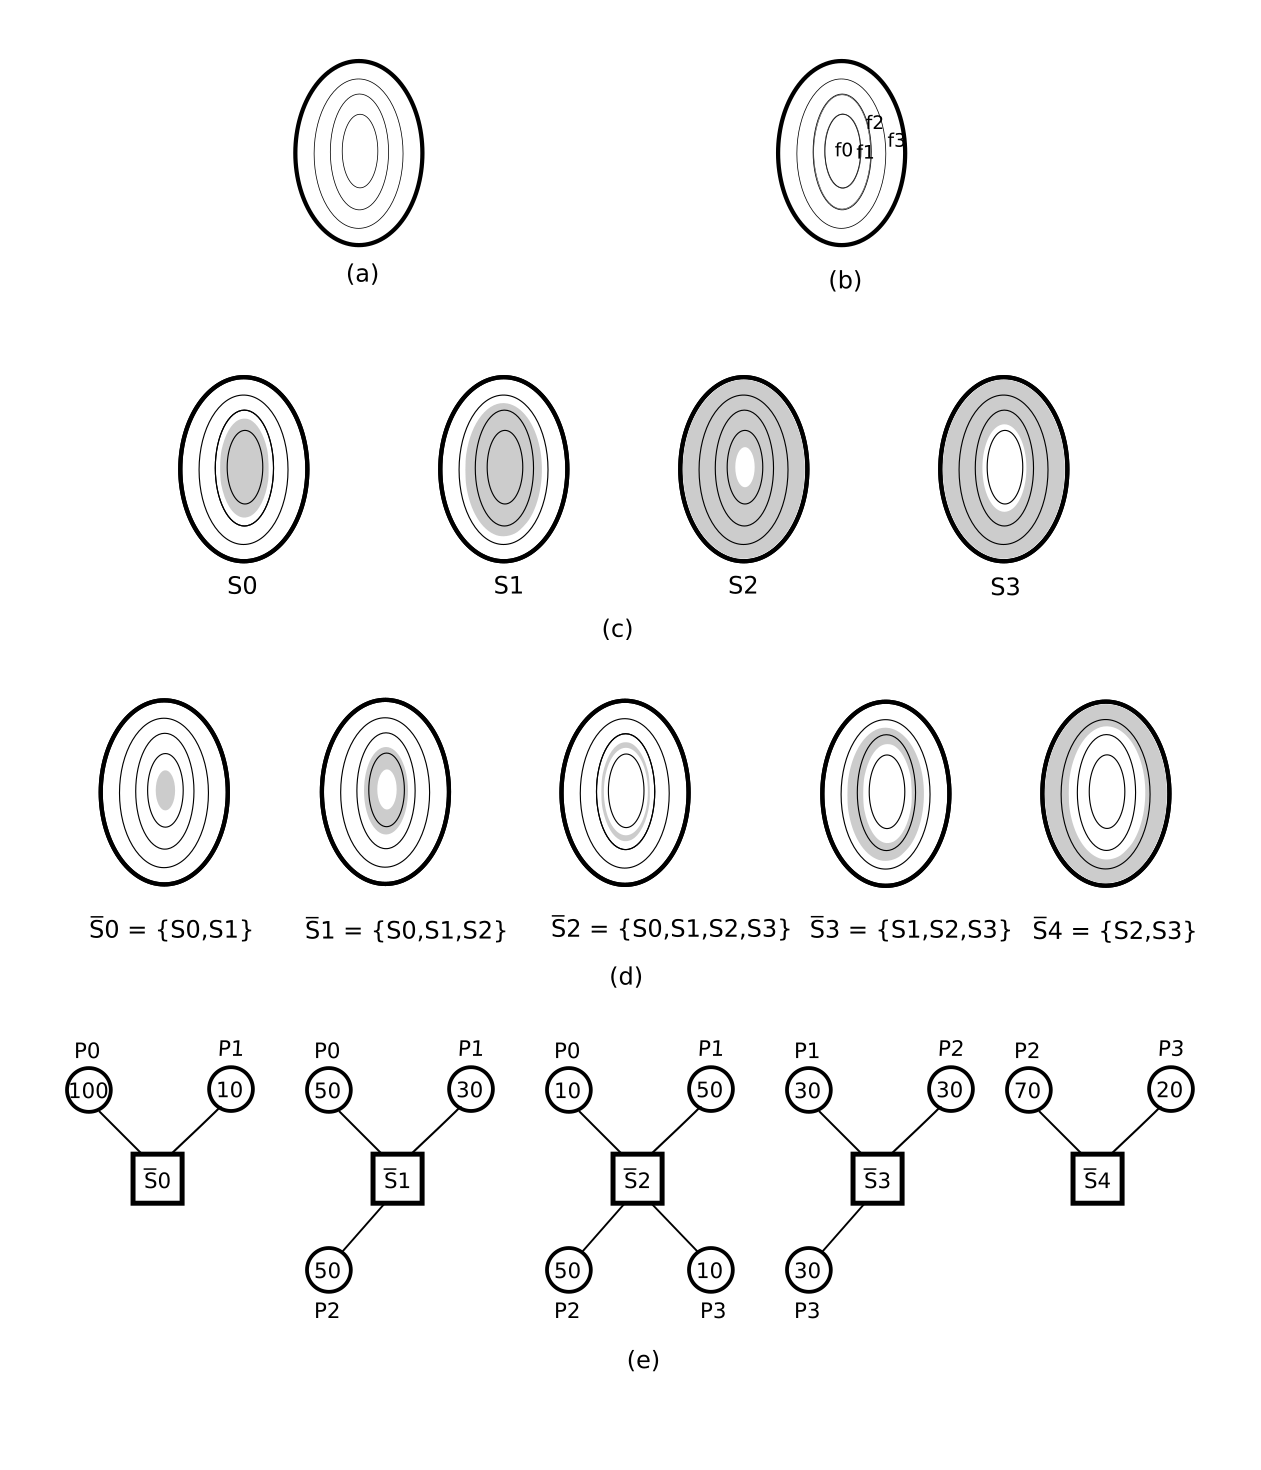
\includegraphics[width=.4\textwidth]{../figures/xgcm_ngraph_construction.png}
  \caption{An example of overlapping safe zones and the N-graph constructed from them.}
  \label{fig:sbars}
\end{figure}

In order to load balance this graph, we run diffusive techniques on the weights of the vertices
rather than the vertices. This means that instead of migrating graph vertices, we migrate the
weight of the vertices across hyperedges to reduce the imbalance of load in the graph.

After EnGPar's weight diffusion is run, a migration plan is returned that details how
much weight to send from each graph vertex on a part to each of its neighboring vertices.
In XGCm, particles are migrated in order to match the plan.

{\color{red} CWS Initial ideas for 'results'}
Since XGCm is still in development, large test cases are not ready. So far two (hopefully)
development
cases have been run showing promising results. The first case has around four thousand
mesh faces, four flux faces and sixteen thousand particles. For this case, EnGPar brings the
initial particle imbalance of 42\% down to 18\%.
The second mesh has 350k elements, X flux faces and YYY particles. EnGPar brings the
particle imbalance from AA\% to BB\%.

\section{Computational Fluid Dynamics}

\begin{itemize}
\item Briefly discuss CFD (FUN3D).
%\item Discuss vertex-based partition vs. element-based partition.
%\item Discuss how EnGPar/Ngraph can support vertex partitions.
%\item Discuss the current approach in FUN3D for partitioning and our ideas to improve it.
\item Mention the boundary stack and our approach to better represent it.
\end{itemize}

{\color{red} CWS Double check this paragraph is OK}
Computational Fluid Dynamic (CFD) applications use meshes in various different ways to solve
problems. One such application, uses finite volume methods on a vertex-partitioned mesh to
{\color{red} CWS list the kind of problems FUN3D solves}. A vertex-partitioned mesh means that
instead of elements being uniquely assigned to parts, the vertices are and the elements are
cut or copied along the boundary to any process that shares them. This application also exhibits
boundary layer stacks where along geometric model faces there are prism elements that are stacked
for a certain distance as well as pyramids at the ends of the boundary layer stacks. Both the
vertex-partition of the mesh and the boundary stacks are challenges for creating a good partition
of the mesh.

{\color{red} CWS (if you have a good one in mind) Show a good boundary layer stack mesh}

Currently for the application, partitioning is done by running (Par)METIS on the graph created
from mesh vertices and mesh edges. As normally seen from multilevel graph
partitioning [REFERENCES],
the vertices are partitioned well, but the mesh edges and mesh elements have a large
imbalance which are key components of the computational load. We improve the imbalance of
mesh edges and mesh elements using EnGPar's diffusive load balancing method.

\subsection{Vertex-partitioned meshes}

To represent the vertex-partitioned mesh in EnGPar, the construction
is essentially the opposite of the element-partitioned mesh. Graph
vertices are defined by mesh vertices and graph hyperedges are defined
by mesh elements. The pins between graph vertices and hyperedges are
created for any mesh vertex that bounds a mesh element.
{\color{red} The following line can be removed if we don't do this.}
Additionally, a second edge type is used for mesh edges where each
hyperedge would have pins to the two mesh vertices that bound the mesh edge.

{\color{red} Add a figure of vertex-partitioned mesh to Ngraph?}

During initial attempts at improving the partitions, we found that the edge cut was growing
at a large rate as we improved edge imbalance. This has been attributed to the differences
caused by the vertex-partitioning of the mesh. For element-partitioned meshes, the hyperedges
represent the mesh vertices. To maintain a low edge cut, mesh vertices that bound many mesh
elements should not be cut across partitions. Towards this, EnGPar avoids migrating cavities
around these high-degree hyperedges. For vertex-partitioned meshes, this problem is reveresed
since mesh vertices are represented as graph vertices and hyperedges all have roughtly uniform
low degrees based on the element: four in a tetrahedron, five in a pyramid, six in a prism, etc.
Thus the problem of edge cut arises for having high degree graph vertices along the partition
boundary which leads to a larger edge cut.

To control the edge cut while balancing the graph, we introduce a metric to represent the
potential edge cut change for a cavity. The metric is the ratio of hyperedges that will be cut
after the cavity is migrated to the hyperedges currently cut around the cavity. We introduce a
parameter to EnGPar that will only migrate a cavity if the metric is below the given tolerance.
Setting this parameter to 1.0 forces EnGPar to migrate cavities that will not increase the edge
cut locally. This does not guarentee that the edge cut will decrease as the metric does not take
into account other cavities that are migrated in the iteration. Smaller values of this
paramter will limit the increase in edge cut, but also limit EnGPar's ability to improve the
imbalance and either take more iterations to reach the imbalance tolerance or stagnate at a
higher imbalance.

\subsection{Boundary Layer Stacks}

{\color{red} CWS I think the following sentence is true?}
For the CFD application, it is ideal to partition boundary layer stacks such that each stack
is on a single process. However, without explicit information, graph partitioners will cut
the boundary stacks up including EnGPar's diffusive load balancer. In order to keep boundary
stacks together on a process, we combine the mesh vertices of each stack into one graph vertex
during construction of the N-graph. Algorithm \ref{alg:collapse} details steps taken to
combine the stacks. To maintain the correct computational and communication load of the stacks,
we attach weights to the vertices and hyperedges that result from the stack. Each boundary layer
stack vertex is given a weight equal to the number of vertices in the stack, and the hyperedges
are given a weight of the number of elements that share the same graph vertices. All other
graph vertices and hyperedges are given a weight of one.

{\color{red} Boundary stack collapse algorithm}

\section{Results}
\begin{itemize}
\item PIC
\begin{itemize}
  \item engpar vs no balancing timing and particle imbalance
\end{itemize}
\item FUN3D
\begin{itemize}
  \item with and without BL collapse
  \item engpar parmetis (no BL collapse) vs fun3d parmetis(?) - may not be
    possible without help from eric - need fun3d solver counts of vertices to
    compute its imbalance
  \item engpar parmetis (no BL collapse) + vtx improvement vs engpar parmetis
  \item engpar parmetis (no BL collapse) + vtx > elm improvement vs engpar parmetis
\end{itemize}
\end{itemize}

Experiments for the vertex-partitioned mesh application were done with a 60 million
element mesh on 1024 to 8192 processes. To show the affect of the edge cut
metric, we ran the same test for each process count giving values for the metric
from 0.5 to 2.0 as well as the metric being turned off. Each test runs 30 iterations
of EnGPar's edge balancer while strictly maintaining the vertex imbalance. Figures
\ref{fig:metric_cut} and \ref{fig:metric_imb} show the edge cut and edge imbalances for each
test. The initial stats after parmetis has partitioned the mesh is also provided. Without
the metric used, EnGPar reduces the edge imbalance by XX\% while increasing the cut by
XX\%. {\color{red} Add more discussion about the results.}

For the boundary layer collapse, we use the same 60 million element mesh. The N-graph is
built in serial from the mesh with and without
collapsed boundary layers and partitioned out using global parmetis for the 1024 to 8192 partitions.
Then, EnGPar is run for 30 iterations to reduce the edge imbalance. Figures \ref{fig:collapse_cut} and
\ref{fig:collapse_imb} show the edge cut and edge imbalance after partitioning with
parmetis and after EnGPar. {\color{red} Insert discussion about the results.} 

\section{Closing Remarks}
foo

\begin{itemize}
\item accelerators
\item BL collapse
\end{itemize}

\bibliographystyle{IEEEtran}
\bibliography{scorec-refs/scorec-refs}

\end{document}
